
\section{The Phase II Project}
\label{sec:phaseII}
%% {\em Provide an explicit, detailed description of the Phase I research
%%   approach and work to be performed.  Indicate what will be done, by
%%   whom (small business, subcontractors, research institution, or
%%   consultants), where it will be done, and how the work will be
%%   carried out.  If applicant is making a commercial or in-kind
%%   contribution to the project, please describe in detail here.  The
%%   Phase I effort should attempt to determine the technical feasibility
%%   of the proposed concept which, if successful, would provide a firm
%%   basis for the Phase II grant application.

%%   Relate the work plan to the objectives of the proposed project.
%%   Discuss the methods planned to achieve each objective or task
%%   explicitly and in detail.  This section should be a substantial
%%   portion of the total grant application.} 

\subsection{Technical Objectives}
%% {\em State the specific technical objectives of the Phase I effort,
%%   including the questions it will try to answer to determine the
%%   feasibility of the proposed approach.}

The requirements being addressed include the development of a native web
workbench for the nuclear engineering community to encourage the adoption of 
state-of-the-art modeling software that are continually being developed under 
government funded programs such as NEAMS. 

In Phase II, RNET Technologies and ORNL will pursue the following objectives:

\begin{enumerate}

\item \rnetprop{Develop the core CloudBench features, such as dynamic, human-in-the-loop workflow editing, 
provenance model creation, and sharing of workflows and/or computed results. The develop of these features will form the core of CloudBench, and are therefore executed to consume the bulk of the Phase II development effort.
This will involve the development of dynamic ``drag-and-drop'' components to 
represent workflows, the validation of imported workflows, and dependency 
resolution for imported workflows. This in turn will feed the development of provenance-based 
workflows by assisting in the recording of actions and configurations. Finally, 
we will add support for the sharing of workflows.}

\item \rnetprop{Develop and demonstrate full Cloud Integration for remote simulation execution on clouds and HPC clusters. Initial development will focus on a well known Cloud API (e.g., AWS). It is important 
to develop a seamless and transparent interaction layer with cloud service 
providers. This interaction is responsible for spinning 
up instances for execution, calculating and tracking costs as they accumulate, 
harnessing storage services, etc. Not only will this encourage the usage of 
various codes, it will also abstract away most of the details of having to 
interact with the Cloud-based services.}

\item \rnetprop{Prototype, integrate, and demonstrate web based Remote
  Visualization integrated into the CloudBench workbench. Initial
  efforts will use pre-generated data (e.g., a Nek5000 test case) for
  development and testing. The infrastructure will be developed using
  input from ORNL on EAVP and embedding VisIt or ParaView as needed.}

\item \rnetprop{Develop support for several NE based applications from
  the NEAMS toolkit.}

%% \item \rnetprop{Implement an Authentication Framework since CloudBench would 
%% also support interacting with sensitive workloads on AWSGovCloud. The framework will provide users access to workflows, tools, and remote storage. CloudBench will only store workflow and provenance information internally (which will be protected by the CloudBench credentials), all remote simulations and data will be protected by both the CloudBench credentials and the native access policy of the resource (e.g., the file system policy enforced via ssh access). Providing and 
%% reusing  supplied credentials (whenever appropriate) is crucial towards being 
%% able to execute and obtain results from sensitive workloads. It is expected that the user will be required to enter credentials for remote utilities each time they are invoked (including two-factor authentication). By using 
%% CloudBench, users will explicitly agrees with the Terms of Use which will prohibit 
%% sharing or access of export-controlled information through CloudBench.}

%\item \rnetprop{Implement and verify proposed Tiered Fee model. This is 
%necessary to ensure that the User is rightfully informed of charges associated 
%with using CloudBench and that RNET's share is also accurately obtained. 
%Correctly calculating these costs and presenting the user with breakdown 
%ensures trust which is critical for the success of the platform.}

\end{enumerate}

\subsection{Work Plan}
\label{sec:workplan}
\subsubsection{CloudBench Architecture}

\begin{figure}[thb]
\begin{center}
\leavevmode
\includegraphics[width=0.7\linewidth]{./narrative/figures/cloudbench_workflow.jpg}
\end{center}
\caption{User perspective of CloudBench.}
\label{fig:cloudbench_workflow}
\end{figure}

A User's view of CloudBench features is shown in 
Figure~\ref{fig:cloudbench_workflow}. This figure outlines our intended aims of 
interacting with various clusters, performing remote simulations and 
visualizations, developing a workflow-based provenance and sharing it amongst 
other users. In order to support this, our proposed architecture is as shown in 
Figure \ref{fig:arch}.

%\begin{wrapfigure}{r}{0.65\linewidth}%[thb]
\begin{figure}[thb]
\begin{center}
\leavevmode
\includegraphics[width=0.7\linewidth]{./narrative/figures/product_arch.png}
\end{center}
\caption{Overall framework for CloudBench (leveraging Vaadin~\cite{vaadin_client_app}).}
\label{fig:arch}
\end{figure}

CloudBench is built using Vaadin~\cite{vaadin} and is fundamentally a web UI 
front end for interactive workflow development, visualization, provenance,
sharing, and remote and local job execution (built over Eclipse ICE
for remote job management). CloudBench can be run on a hosted
environment or a private server. CloudBench can be modified to support
a wide range of large scale numeric applications to support various
niche simulation industries (including Nuclear Energy).

Vaadin is a particularly adept tool at creating web-based portable
applications using Java. The underlying details of representing pages
and components (specified with Java) using HTML, CSS or Java-script is
conveniently handled by the Vaadin framework. CloudBench is aimed to
be designed as a Server-Side application which can connect to a Server
where a ``Core'' instance will exist. The Server instance
could be the local machine, a cloud-based instance, or a traditional
HPC architecture to allow convenient access to higher performance
instances. CloudBench will also benefit directly from Vaadin's Security 
Model~\cite{vaadin_security} which follows good security practices and provides 
automatic protection against Cross-Site Scripting (XSS), Cross-Site Request 
Forgery (XSRF) and other methods. Finally, CloudBench will further leverage the 
communication layer provided by Vaadin and use OSGi services similar to the ICE
architecture to handle remote instances.

%{\lfoot{\small{May contain trade secrets or commercial or financial\\ 
%information that is privileged or confidential and exempt from public 
%disclosure.}}} \afterpage{\lfoot{}}

A typical CloudBench simulation is shown in 
Figure~\ref{fig:cloudbench_simulation}. The Core instance runs on a Cloud (or 
HPC, or 
Local) instance and reads input data from an appropriate source (a local (parallel) filesystem, a remote GridFTP copy, 
cloud storage access such as S3). The simulation is executed with the relevant computational tool 
and the output data is post-processed remotely as shown in 
Figure~\ref{fig:cloudbench_simulation}. Each of the steps are recorded as part 
of 
the provenance model (see shown in Figure~\ref{fig:workflow_provenance}).

%\begin{figure}[thb]
%\begin{center}
%\leavevmode
%\includegraphics[width=0.8\linewidth]{./narrative/figures/cloudbench_workflow.jpg}
%\end{center}
%\caption{CloudBench Workflow with various stages.}
%\label{fig:cloudbench_workflow}
%\end{figure}
%
%\begin{figure}[thb]
%\begin{center}
%\leavevmode
%\includegraphics[width=0.3\linewidth]{./narrative/figures/workflow_provenance.jpg}
%\end{center}
%\caption{Growth of provenance model with steps.}
%\label{fig:workflow_provenance}
%\end{figure}

%\begin{figure}[thb]
%  % Fixed length
%  \centering
%  \leavevmode
%  \subcaptionbox{CloudBench Workflow.\label{fig:cloudbench_workflow}}  
%{\includegraphics[width=0.2\linewidth]{./narrative/figures/cloudbench_workflow.jpg}}\hspace{1em}%
%
%  \subcaptionbox{Corresponding Provenance.\label{fig:workflow_provenance}}  
%{\includegraphics[width=0.2\linewidth]{./narrative/figures/workflow_provenance.jpg}}
%\end{figure}

\begin{figure}[thb]
\centering
\begin{minipage}{.6\textwidth}
  \centering
  \includegraphics[width=\linewidth]{./narrative/figures/cloudbench_simulation.jpg}
  \caption{CloudBench Simulation with various stages.}
  \label{fig:cloudbench_simulation}
\end{minipage}%
\begin{minipage}{.4\textwidth}
  \centering
  \includegraphics[width=.5\linewidth]{./narrative/figures/workflow_provenance.jpg}
  \caption{Growth of provenance model.}
  \label{fig:workflow_provenance}
\end{minipage}
\end{figure}

%\rnetcomment{Paragraph below does not make sense to me. What
%  existing web services? What storage services? Is this a carryover
%  from the Phase I that needs to be deleted? -- Jerry}
%
%The architecture in Figure~\ref{fig:arch} relies on the existing web services 
%and eliminates the extra effort required 
%for developing specialized storage services, discussion forums etc. for 
%creating a custom web portal. By basing our portal 
%on the Restful API, the future web services can also be easily integrated into 
%the portal. The Restful APIs are used by 
%multitude of websites including cloud companies (Google, Amazon etc.), project 
%hosting websites (Github, SourceForge etc.), 
%and social networking websites (LinkedIn, Facebook etc.). Using this API, 
%these websites allow the users to programatically 
%search through the hosted software,interact with the cloud services, and 
%posting and retrieving social networking feeds.

\subsubsection{Cloud Integration}
\label{sec:cloudinteg}

% TODO: Develop fig to outline interacting with various Cloud-based services.

%\begin{figure}[thb]
%\begin{center}
%\leavevmode
%\includegraphics[width=.9\linewidth]{./narrative/figures/WarthogInICE.png}
%\end{center}
%\caption{NiCE running the Warthog application from NEAMS showing problem setup 
%and solution visualization.}
%\label{fig:ice}
%\end{figure}

% why focus on cloud integration?
Increasingly, cloud-computing clusters are becoming a viable alternative to 
access high-performance instances (higher memory, more number of cores, etc.) at 
a nominal cost. Especially with services like AWS, Microsoft Azure and Google 
Cloud, such instances can be spun up within minutes and can transparently 
provide timely backups and reliable storage. For some use cases (jobs requiring upto about 25,000 cores) applications, users may often 
find that their local systems are busy with existing jobs or become outdated 
due to technological trends. In some cases, it is desirable to execute relevant 
simulations on the cloud cluster due to the immediate access to up-to-date 
hardware and availability of systems. In addition, many commercial and academic users will prefer to use public clusters without the upfront cost and ongoing maintenance requirements.

CloudBench will be able to interface with various clouds, including public clouds (e.g., AWS) and private Clouds (e.g., ORNL's CADES)  and HPC clusters.
To support this integration, CloudBench uses a unified framework for 
authenticating to various entities. The proposed unified framework will safely 
store user credentials for interactions between various systems. It will prompt 
for credentials when required and will renounce authenticated tokens or 
resources when no longer needed.
% Complete along the lines of "that's why cloud integration is important and so 
%on."
Under the hood, CloudBench will use ICE for remote job management. ICE will manage authentication and storage for remote execution. ICE handles authentication using the Secure SHell (SSH) Protocol (among others) and stores credentials in a fully encrypted local storage for reuse. (Note that this can be customized too, for example, avoid storing credentials to remote machines on a server.) Therefore, the underlying system security model will continue to be enforced when accessing remote data and simulation tools.

Some of the nuclear engineering software in the NEAMS toolkit have
licensing and export control concerns that prohibit general cloud deployment, especially
for tools like BISON and PROTEUS. In addition, even if the tools
themselves do not have any license or export control limitations, the application
of the codes to a particular problem may invoke export control
limitations. In order to overcome the export control and licensing
issues, we will identify and leverage the cloud services that meet the
government regulatory and compliance requirements (NASA Nebula, AWS
GovCloud, Nimbis Services etc.). Access to remote tools and remote data will be limited by CloudBench, but will also be enforced by the remote system (e.g., access to files will be restricted by the standard file system access controls via ssh and/or GridFTP). Workflow and provenance information will be the only data stored natively in CloudBench. Native data will be protected from third-party access, and the user will have full control over which (if any) users have access to a workflow or provenance history (users will agree to an EULA that prohibits sharing export controlled data with unauthorized users). Further, we will require users to
obtain licenses from the relevant software groups before providing
access to hosted tools or datasets via CloudBench. Where feasible, we
will develop protocols to help mediate between the application providers and the
end users to assist in the licensing process (i.e., identify points of contacts, assist in obtaining
forms, following up on requests, etc.).

In addition to hosting CloudBench on export controlled compliant Clouds
and ensuring access is granted by the appropriate licensing group,
RNET will support the deployment of a CloudBench server on internal
machines, websites, clusters, and private clouds. This will provide
complete access control to the hosting entity (e.g., a government
research group or a commercial company).

%% The execution of export controlled code needs to be considered from two perspectives: the execution of software installed alongside CloudBench and the execution of third-party software provided by users that is not part of CloudBench. In the first case, CloudBench will support all necessary controls and access restrictions. For the second case, CloudBench can only rely on the access privileges granted by the third-party system.

% Talk about Authentication and how we want to handle.
%\subsection{Authentication}
% Explore avenues to interface to various handlers? OAuth2? What does it do and 
%how will it interact?

%\subsection{Handling ITAR}

%The CF configuration files are provided in JSON format, where all resources 
%that need to be provisioned (such as 
%EC2 instances, policies, network connections and subnet, etc.) are listed. In 
%addition input parameters can be 
%stated for user to potentially supply input, such as the size of cluster, etc. 
%An S3 bucket is also provided 
%that includes scripts and files that are needed to be loaded on EC2 instances, 
%once they are set up. We can use 
%this bucket to include our pre-configuration, dependency installation, 
%compilation and execution scripts. Another 
%S3 bucket can be used to download the output results at the backend. 
%
%A drawback to this approach is that the Cloud setup may be long, more than 10 
%minutes. To overcome this issue, 
%in the back-end, we will cache the Cloud for future usages by the same user. 
%The users need to pay for the Cloud 
%idle time, if they choose to have a persistent Cloud throughout their login 
%session. 
%
%For simple calculations, technologies like AWS Lambda can be leveraged to 
%automatically scale the 
%embarrassingly parallel binary applications to the available cloud computing 
%resources. With Amazon Lambda, 
%unlike other AWS services, there is no need to create compute instances and 
%install the required software 
%stack for launching the applications. Arbitrary executables written in any 
%language can be run in the cloud 
%by creating Lambda functions. For the purpose of our web portal, ready-made 
%binaries that run in the cloud 
%can be developed using AWS Lambda to ease the deployment and management cloud 
%for domain scientists. 

\subsubsection{Provenance \& Sharing of Data}
\textbf{Workflow and Provenance}
\label{subsec:provenance}

% Why is provenance important?
A {\em simulation} typically consists of an input model and solver
preferences/settings, followed by post-processing and visualization
efforts. It is often very desirable to study the effect of changing
the design, modifying a parameter(s) and evaluating the effect in an
incremental manner. A {\em workflow} consists of several such
simulations chained together to transform an initial input into a
final desired output. In between simulation steps, tools and scripts
may need to be used to reformat/remesh data to allow integration of
otherwise disparate tools.

In some domains, a workflow is a static entity that is used to combine
several simulation tools into an aggregate tool to perform a specific
task. In NE and many other scientific and research oriented
applications, the workflow is dynamic and requires a {\em
  human-in-the-loop}. The researchers and team members know which class of applications
that are going to be required, but the specific applications required
and the simulation inputs are not known until the previous stage is
completed and the human can evaluate the output. Additionally,
sometimes a given stage needs to be executed several times to either
develop alternative solutions or to refine a stage (possible after
later stages have completed). Further, sometimes the simulations are
explorative, and the intermediate results are not historical important
when sharing a final workflow that a third-party scientist can use to
confirm a simulation or as a baseline for new experiments. This is particularly true in licensing applications where each task is signed off by a human and passed to the next in the chain.

Therefore, the workflow development environment needs to be
dynamic. Users need to be able to setup workflows, pause workflows,
and edit/add steps in the workflow. Further, the user should be able
to use the existing workflow and history (i.e., notebook) to create a
sharable workflow.

This leads to complex simulation 
histories. Therefore, attempting to manually track and maintaining a link between results obtained earlier and the 
corresponding problem setup is often error prone and cumbersome.

%In CloudBench, we expect a particular workflow (e.g., using NE tool such as  
%NEAMS tools in this example) to proceed in a manner as shown in 
%Figure~\ref{fig:prov_workflow}:

%\begin{figure}[thb]
%\begin{center}
%\leavevmode
%\includegraphics[width=0.7\linewidth]{./narrative/figures/provenance_workflow.png}
%\end{center}
%\caption{Sample Workflow in CloudBench:NE.}
%\label{fig:prov_workflow}
%\end{figure}

The workflow can be represented as a simple Directed Acyclic Graph (DAG). A 
typical workflow would involve calling multiple solvers for a multi-scale 
simulation and conducting post-processing efforts at various stages of 
the simulation. Reliably reproducing this workflow is crucial towards 
validating the efficacy of any particular model, and when using a past simulation workflow to iteratively design a new simulation. This is particularly true when 
results differ after sharing workflows among other members or collaborators (or a regulator). 
Various factors can cause the calculated results to differ from the recorded 
results, ranging from different software versions, differing hardware 
configuration and errors in problem setup. So it is imperative to develop a 
system that allows for the accurate recording of relevant measures to ensure 
that results can be duplicated, verified, and extended. The CloudBench workflow and
provenance model is based on the Open Provenance Model (OPM). This models meets the following requirements ~\cite{open_provenance_spec}:

\begin{enumerate}
\item Allowing provenance information to be exchanged between systems.
\item Allowing developers to build and share tools that operate on such a model.
\item Defining provenance in a precise manner.
\item Supporting a digital representation of provenance for any suitable object.
\item Allowing multiple levels of descriptions to exist.
\item Defining a core set of rules that identify the valid inferences that can 
be made on provenance information.
\end{enumerate}

The CloudBench framework records provenance of a simulation workflow using an
XML format to ensure that it can be parsed conveniently as part of result 
files. A typical provenance record details such as:

\begin{enumerate}
\item Version Record: This would include the version of CloudBench, scripts, applications being used, and compiler time information. 
For particular NEAMS codes/tools, we would record an appropriate ID based on 
the version control being used (e.g., GitHub: SHA-1 ID of the code or Subversion: SVN commit ID).
  
\item Compiler options: Flags and switches specified while using a compiler or 
runtime arguments for a Java VM or Python interpreter as well as its version.

\item Hardware configuration: Clock speed of the processor, Architecture 
codename (like Skylake, Haswell, etc.), number of threads supported, total 
memory, network, etc.
\item Date and time.
\end{enumerate}


We will support suitable readers and writers that can parse provenance data (which will normally be hidden from the user, unless it is exported to an XML file to be used externally to CloudBench). 
Result files generated using CloudBench will include this provenance setup. 
When read by CloudBench, options will be exposed that will let the user decide 
whether to fetch appropriate codes based on the version numbers stored (as 
shown in Figure~\ref{fig:prov_workflow_with_vers}) and automatically compile 
them using the compiler version and options (if compile versions do not already exist).

\begin{figure}[thb]
\begin{center}
\leavevmode
\includegraphics[width=0.6\linewidth]{./narrative/figures/provenance_workflow_with_vers.png}
\end{center}
\caption{Sample Workflow in CloudBench:NE with Versioning Information.}
\label{fig:prov_workflow_with_vers}
\end{figure}

Further, a User might work with a workflow, modify them and ``Save'' them to 
form a new workflow. It would be very useful to preserve this history in a 
linear fashion so that Users may know the ``Original'' version and get an 
idea as to how the workflow has evolved as shown in 
Figure~\ref{fig:prov_workflow_linear}.

\begin{wrapfigure}{r}{0.5\linewidth}%[thb]
% %\begin{figure}[thb]
\begin{center}
\leavevmode
\includegraphics[width=0.7\linewidth]{./narrative/figures/provenance_linear_history.png}
\end{center}
\caption{Linear History of Provenance.}
\label{fig:prov_workflow_linear}
\end{wrapfigure}

\textbf{Sharing}
\label{subsec:sharing}
%\rnetcomment{Jay -- Discuss export here}
% Talk about how data will be shared. Permission issues.
Provenance is particularly appropriate when sharing results among 
collaborators. CloudBench will include a suitable framework that 
allows sharing of results among a group of related users. Particularly, we need 
to handle sharing of results that may contain export-controlled information. 
The policy in CloudBench will be to consider an entire workflow as restricted 
 if any of the components are export controlled. The full set of CloudBench policies on export controlled data and software will be outlined in the CloudBench End User License Agreement (EULA).

The user and group features provided in CloudBench will be a facade to
the backend filesystem, and access control will be provided by the
backend filesystem and system security.

%% When another user is specified to receive the data 
%% (assuming export controlled restrictions have been handled as described 
%% earlier), then appropriate permissions are set on the shared data space for the 
%% data to be visible to the user. Then copies of the shared data can be made (if 
%% needed) and the originator can choose to revoke sharing at any time.

%% If the instance is local or no traditional cloud service provider is used, we 
%% will also support a point-to-point sharing method, either by using GridFTP 
%% (\rnetcomment{Does this make sense?}) or using Secure Shell Copy 
%% (\rnetcomment{This requires that a common user acct be available on source and 
%% destination systems with read permissions on the data. What about multi-share? 
%% Gets complicated.})

%We envision the Results file as being composed of:

%% \rnetcomment{Jay, thoughts on sharing and export control in this section? Having
%%   non-export and export controlled data in a single project seems to
%%   sensitive to me. I think I would prefer an arraignment that is more 
%%   stringent. If any tools are used that include export controlled data, the 
%%   entire workflow is export controlled. Does it make sense to have ``classes of 
%%   export controlled'' users to restrict access? Additionally, users can mark 
%%   workflows as export controlled (make it the default?). Maybe this is handled 
%%   by the end user, we give a list of all users, they select who to share with, 
%%   they make the decision on who is allowed? Would that be acceptable? --Jerry}

%\begin{enumerate}
%\item Provenance Information: As described in Section~\ref{subsec:provenance}.
%\item Results Section:
%  \begin{itemize}
%  \item Non-export Controlled Data: Accessible to all users with sharing 
%  permissions.
%  \item Export-Controlled Data: Availability will depend on credentials 
%  provided by the User.
%  \end{itemize}
%\end{enumerate}

%\rnetcomment{What is an ``authentication credential''. Export control
%  level (I do not know what that means specifically) and
%  code/data/workflow it is associated with?}
%
%% ITAR sensitivity?
%A typical User profile will include information on which groups they are a 
%part 
%of as well as authenticated credentials for access to Export-Controlled Data. 
%We will store these in Secure and well-tested databases, possibly hosted on 
%Cloud clusters (for additional security). In cases where the sensitive data 
%itself might need fine-grained access, based on the security clearance of the 
%individual, we will leverage available APIs and tools that allow ITAR based 
%authentication. % TODO: Check and document these APIs.
%\rnetcomment{I think I recommend only coarse permissions, and default on 
%restricting. If a workflow contains any sensitive info, the entire thing is 
%off 
%limits. If a user wants to share with a non-export control person, they MUST 
%create a new workflow that does not contain any export control info. What is 
%shared must be crystal clear.}

%% Like any sharing-based system, we will support the following features:

%% \begin{enumerate}
%% \item Creating a group of users.
%% \item Providing sharing permissions for a results file to any particular 
%% user/group.
%% \item Adding an existing user to a group and updating permissions on results 
%% already part of the group.
%% \end{enumerate}

%% \rnetcomment{Jay, lets discuss so Ram or I can take a crack at this Monday morning. Where is shared data stored? How is it shared across sites? Simulation input/output stored on the machine they are used on? Simulation setup and workflow info, and visualization output stored in CloudBench webserver? Utilize host system permissions to restrict access? Need to discuss data transfer when executing a shared simulation, i.e., user can select to transfer a non-local dataset or point to an alternate local dataset. -- Jerry}

% Input decks.
% Recording provenance, sequence of actions, sharing workflows.

% Do remote visualizations?
% What can we leverage for this?
% Transferring data might be costly. Remote rendering might be slow OR would it?
% Today we can stream game graphics onto a thin client, allowing the server to 
%do the rendering. Surely we can leverage this technology for post-processing? 
%Look at EnginFrame from NICE (not ICE related).
\subsubsection{Visualization}
Post-processing of results is crucial to identify potential areas of 
improvements and the effect of parameters on the simulation. When CloudBench is 
connected to a ``Core'' instance on the Local Machine, visualization tools will 
be executed as expected on the local instance. Since data and post-processing 
calculations occur on the same machine, there is no latency in processing.

%% \rnetcomment{Jay, Can/should we leverage your Eclipse Advanced
%%   Visualization Project? Can you improve this writeup based on that
%%   experience? -- Jerry}

When the Core instance is on a remote machine however, the
computational tool executes and produces the output data on the remote
instance. To post-process this, users traditionally have two options:

\begin{enumerate}
\item Move the data to the client machine and post-process
  locally, to improve the interactive response times when exploring the data. This is typically costly, due to the size of the data being
  transferred. Large scale simulations can output data of the order of
  terabytes. Not only is the data transfer time consuming, but cloud
  computing resources charge for the data being transferred, based on
  the total size.

\item Post-process on the server machine. This avoids the data
  transfer costs, but typically this results in slow response times
  when interactively exploring the results, result in recalculations
  and re-rendering, causing delays.
\end{enumerate}

This is a problem that has been seen before but has been well solved 
by various efforts in tools like ICE by leveraging tools such as  VisIt, ParaView and the Eclipse Advanced 
Visualization Project (EAVP). Remote Visualization is realized through the use 
of a thin client process which connects to a server located on a high 
performance machine, which might support GPU rendering. Remote visualization is 
also expected to be the future in HPC since datasets will continue to grow in 
size~\cite{hpc_remote_viz}. Further, this will ensure portability by ensuring 
that the viewing device has to only display the final result (which can be saved in a workflow provenance history).

Modern day cloud-gaming services (such as PlayStation Now and NVidia's 
GeForce Now) have perhaps taken this further. In such a service, the relevant 
games are loaded and rendered on a remote server and the final rendered frames 
are streamed to the User. Interactions such as changing directions or 
keystrokes are minimal updates and are sent in real-time with the response time 
being low enough that these are viable commercial services. One can imagine 
that rendering frames in a highly dynamic environment (user input, multiple 
users, network play, etc.) such as the latest 3D games must be significantly 
challenging, but well handled.

CloudBench will leverage advancement in these areas, and particularly in EAVP, to support efficient Remote 
Viewing. When the ``Core'' instance is on a remote instance, the framework will 
ensure up-to-date and near real-time renders and will use the GPUs in the 
cluster, if available by utilizing the appropriate remove visualization service in EAVP (i.e. - connections to VisIt, Paraview, etc.), which will then manage the transfer of data between the remove visualization cluster, the backend workflow server running the Core and the client. 

%The ideal way to handle remote visualization would be to keep the data and 
%rendering efforts on the server and only send the final render or a simplified 
%representation of it to the client. This simplified model will represent only 
%the surface geometry and can be cached locally for easier viewing. New 
%post-processing queries will trigger a recalculation and the client can obtain 
%an updated result. Interactions with this model can be represented as simple 
%data (such as desired orientation, zoom level, etc.) and sent to the server to 
%obtain an updated result

\subsubsection{Fee Model}
We will explore various Fee Models to encourage the growth of
CloudBench and to suitably appeal to new users. As discussed in the
Commercialization proposal. The average per user fee is expected to be
\$1,000. We envision a tiered fee model, where an initial free version
will allow basic access for setup, execution, and visualization of
supported open/government sourced codes/applications on local or
private remote compute architectures. Additional tiers will include
support for public Clouds (which will also require a usage fee for
compute resources and data movement), commercial vendor codes,
workflow development, provenance history, and sharing.
% The fee model will also take into
%account the Number of Data sets imported and shared, as well as for
%the Output data sets.

%Implied via sharing, groups, etc.
%ITAR sensitive workloads and sharing will have a higher charge, due to the 
%nature of workloads and for the sharing model. 

CloudBench will use the relevant 
cloud clusters' API for calculating charges based on data movements and 
requests, to keep the User informed and to make decisions based on potential 
transfers of data. On top of the existing fees, RNET will aim to gain a
percentage over the existing costs.% as outlined in Figure~\ref{fig:fee_tiered}.

%%SPACE

%% \begin{wrapfigure}{r}{0.5\linewidth}%[thb]
%% %\begin{wrapfigure}[thb]
%% \begin{center}
%% \leavevmode
%% \includegraphics[width=0.5\linewidth]{./narrative/figures/fee_tiered.png}
%% \end{center}
%% \caption{Tiered Fee Model for CloudBench.}
%% \label{fig:fee_tiered}
%% \end{wrapfigure}

CloudBench will ultimately include support for a wide range of tools and clusters. For CloudBench:NE, the tools in the NEAMS 
toolkit (MOOSE~\cite{moose}, NEK5000~\cite{nek5000} etc.) and CASL will be included for the initial release. The 
users will have the ability to quickly compile these codes and add them to 
their workflow environment for quicker environment setup in any instance. A taxonomy 
for nuclear engineering software that helps identify the relevant software 
based on the simulation problem will also be investigated in Phase II with the 
help of domain scientists.

%The user interface to searching relevant software will be designed to 
%accommodate the users with varying interests 
%and levels of expertise in nuclear engineering. The following questions 
%indicate the type of information that
%can be retrieved from the users with varying levels of expertise. As the users 
%answer such questions, the software 
%found and their details can be dynamically updated in the webpage.
%
%\begin{enumerate}
%\setlength{\itemsep}{0.2pt}
%\item If you anticipate using a parallel machine (e.g., cluster, 
%supercomputer, or cloud), please provide some details 
%(if known) on the configuration such as number of cores, cache hierarchy, 
%accelerators (GPUs etc). 
%\item On which OS(s) do you anticipate using the software? (Linux, Windows, 
%Mac OS)
%\item What input data formats do you want to use?
%\item What input datasets do you plan to use? What is the maximum simulation 
%time you can afford with these datasets?
%
%\end{enumerate}
%
%The nuclear engineering community that can benefit from easy access to 
%predictive modeling software is scattered 
%across government organizations, private institutions, and regulatory bodies. 
%Even though an effective 
%web portal is developed, in these days where the number of registered websites 
%have crossed a billion, it is 
%unrealistic and requires tremendous effort to reach out to the interested 
%parties and get them engaged in the 
%proposed web portal and the associated services. In order to address this 
%issue, we propose to leverage the 
%groups already formed in existing social networking websites and the marketing 
%platforms offered by these websites. 
%For example, searching for ``Nuclear Engineering group'' on LinkedIn results 
%in few groups with a total
%of more than 3000 members. The LinkedIn Ads platform can be used to target 
%such audience based on their job 
%jitle, job function, industry, geography, or the LinkedIn group within a 
%limited budget. In Phase I we will 
%identify several such groups, create sample advertisements, and demonstrate the 
%community engagement using 
%number of views and clicks.
%
%In addition, the existing marketing platforms will also be used to let the 
%users promote their software and 
%results on our portal. The proposed portal will augment the users marketing 
%efforts and help reach the right 
%audience using the local database and past simulations history of the users. 
%The users will be provided with easy 
%interfaces to create advertisements specifically for within the nuclear 
%engineering community. The Facebook API for 
%example provides a programming interface to its advertising platform. Using 
%this feature, a nuclear engineering 
%company (for example, GE Hitachi) will be able to create and publish an 
%advertisement with sample simulation 
%results for a custom reactor. 

In Phase III, we will implement revenue models for on demand simulation using 
popular codes and data sets, private storage of results, and remote 
visualizations. The CloudBench interface will mainly provide a suitable 
framework to work with open-source Scientific Computing and HPC codes. Using 
NEAMS tools, this can be specialized to form CloudBench:NE. A commission will 
be charged on top of the price charged for public cloud computing and storage 
services. 

\subsubsection{Third-party API Integration (e.g., NEAMS Toolkit)}
In addition to the hosted and private server instances of CloudBench,
RNET desires to include support for integration into third-party
tools. Third-party tools would be able to interface with CloudBench
sharing, provenance history, visualization, and remote execution. This will allow
third-party tools to leverage these features, and the community
developed around CloudBench. Integration with the NEAMS Workbench
(being developed within NEAMS) would be a first step along this
route. The goal would be to provide an API that can be called by these
tools. Very preliminary informal discussions were had with the NEAMS
developer, who generally supported the idea of modifying NEAMS to
provide a plugin interface for tools such as CloudBench. This will be
further explored during Phase II.

%\subsection{Other Apps and Databases}
%
%The portal will host a series of other databases and corresponding web 
%applications. Sample applications 
%include searching through the relevant simulation results before embarking on 
%expensive simulations, store 
%the end results of the major findings of the nuclear engineering community, 
%and conversion between different 
%data formats. 
%
%An ``output'' database will be developed to store the simulation results. This 
%database will store the 
%end result of the major findings of the nuclear engineering community. This 
%will allow the community to easily 
%share simulation results. The end user will be able to specify the 
%``visibility'' of the results, allowing 
%them to control if the results are to be shared publicly, within a smaller 
%community/organization, or 
%privately. When the results have been thoroughly validated, the user will be 
%able to submit the results to
%the database if desired.
%
%A ``test case'' database will be developed that includes test datasets and 
%expected results for particular 
%codes. The information stored in the database will include the dataset, 
%meta-data regarding the dataset, 
%dataset format information, and information on the results and performance for 
%a given code. This will 
%allow for the community to share common test cases that can be used for 
%validation and verification, as well as 
%performance comparisons.


%\subsection{Summary of Phase II Goals}
%\label{sec:phaseII}

%Integrate the multitude of project hosting websites, cloud resources, storage 
%services, and other web services.
%Develop high level applications.


\subsection{Performance Schedule and Task Plan}
\label{sec:taskplan}

% Use wrapfigure here instead?
\begin{wrapfigure}{r}{0.5\linewidth}%[thb]
%\begin{figure}[thb]
\begin{center}
\leavevmode
%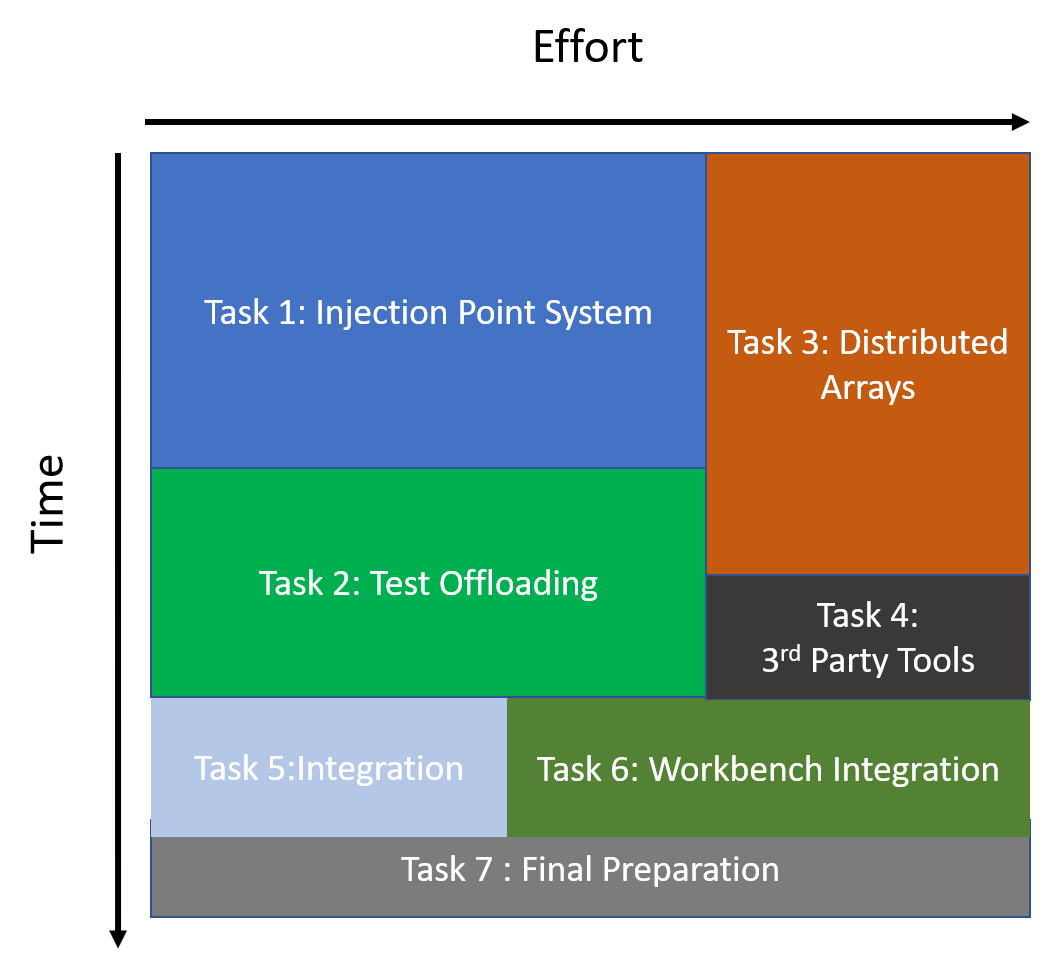
\includegraphics[width=1.0\linewidth]{./narrative/figures/tasks.pdf}
\end{center}
\caption{Overview of task dependencies and timeline.}
\label{fig:tasks}
\end{wrapfigure}

RNET would like to present the project ideas and research plan to the
DOE Program Manager and other interested scientists. The meeting will
be used to discuss features, and identify the specific NEAMS applications and computer
resources that will benefit from this project.  This meeting will be
scheduled soon after the Phase II contract is awarded. The meeting can
be hosted at RNET, a DOE site suggested by the Program Manager or via
a teleconference.

RNET will submit all reports as required by the contract (e.g., annual reports, 
a continuation report, summary reports, and a final report) to the DOE program 
manager and other interested DOE scientists.

The research and development topics described in Section~\ref{sec:workplan} 
will be addressed by the tasks described in the remainder of this section. Most 
tasks require active collaboration between RNET and its collaborators. 
Figure~\ref{fig:tasks} summarizes at a high level the dependencies among tasks  and
approximate anticipated task durations. The duration of the Phase II 
project is 104 weeks. Specific details are included in the description of each 
task.

%RNET would like to present the project ideas and research plan to the DOE 
%Program Manager and other interested scientists involved in the NEAMS program. 
%The meeting will be used to demonstrate the specific software and obtain 
%feedback on the existing CloudBench prototype. This meeting will be scheduled 
%soon after the Phase II contract is awarded. The meeting can be hosted at 
%RNET, 
%a DOE site suggested by the Program Manager or via a teleconference. RNET will 
%submit a final report and present the report details along with 
%a Phase III work plan to the DOE program manager and 
%other interested scientists.


\newcounter{taskCount}
\setcounter{taskCount}{0}

\refstepcounter{taskCount}\label{task:2.5}
\subsubsection{Task \ref{task:2.5}: Develop CloudBench Dynamic Workflow Editing 
Features and Support}
%\rnetcomment{Ram, break this out from task below? I think simulation
%  support and editing workflows is going to be a significant stand
%  alone effort? You have some detail in the workplan, can they be extended 
%here too?}

\rnetprop{\lfoot{}In this task, we will develop methods that will allow a User
  to specify and develop a dynamic workflow DAG. This will involve
  encapsulating basic operations (such as running a simulation using a
  particular tool, transforming/remeshing data, specifying input
  parameters, etc.) as a ``Block''. Available simulations and cluster
  will be stored as objects that the user can select from a predefined
  lists (in addition to adding custom objects as needed). Data objects
  will include URL references to the data and data access
  information. Users will be able to ``drag-and-drop'' these
  entities/objects and specify connections between them as edges. The
  workflow will be editable during execution (e.g., so stages can be
  dynamically removed, added, or edited at each stage in the DAG).  }

\rnetprop{RNET will work on the implementation for this task and ORNL will 
provide inputs and guidance.}


\refstepcounter{taskCount}\label{task:3}
\subsubsection{Task \ref{task:3}: Develop CloudBench Provenance Features}

\rnetprop{Storing the provenance information is crucial towards being able to 
reproduce results or to understand any deviations from the original workflow. Along with the Workflow 
information, we will develop methods that document the configuration used while 
building relevant tools and other information as outlined in 
Section~\ref{subsec:provenance}. This will be stored with the Workflow to form 
an object that can be shared amongst other Users to reliably reproduce results.}

\rnetprop{RNET will work on the implementation for this task and ORNL will 
provide inputs and guidance.}

\refstepcounter{taskCount}\label{task:2}
\subsubsection{Task \ref{task:2}: Develop the Remote Cloud Integration Framework}

\rnetprop{In this task, we will develop an interface that will allow the user to 
select and interact conveniently with a Cloud Computing frameworks like AWS and ORNL CADES. 
We will develop abstractions that leverage the Cloud frameworks' APIs. The User 
will be able to create instances that are automatically configured for 
CloudBench, run simulations, store/retrieve data and precompute related costs 
(such as for data movement).

In addition to the user facing UI, we will develop a modular code interface
to allow the integration to many Cloud and Cluster architectures with
minimal incremental effort. This will allow a wide range of architectures to be supported, and allow RNET to offer contractual post-SBIR services to develop custom integration for CloudBench clients.

We will initially focus on a well developed API (e.g., AWS and CADES)
first and then generalize the developed interfaces to support other cloud 
computing clusters and validate our efforts by running the same workflow in all 
cases. We will also extend this to AWS GovCloud and ensure that controlled 
workloads can be executed.}

\rnetprop{RNET will be responsible for this task. ORNL will provide guidance on 
developing the framework for ORNL CADES.}


\refstepcounter{taskCount}\label{task:4}
\subsubsection{Task \ref{task:4}: Workflows Sharing Interface}
\rnetprop{We will develop methods to support sharing between users by 
allowing the definition of groups. Users and groups in CloudBench will be enforced by both CloudBench and the underlying file system and system security model. For hosted systems, the CloudBench user/group API will be a facade for the cloud system (which will enforce access controls). For remote file systems, the CloudBench API will define access to the workflow description, but the remote filesystem will ultimately restrict access using its native access control mechanisms (e.g., an scp or GridFTP transfer will fail is the user does not have appropriate access on the system, CloudBench will not attempt to alter permissions on remote systems).

%Shared data will be stored in an area that would be accessible 
%to all users within the group. We will validate these efforts by sharing such 
%an object with another User and validating the recalculated results.

This task will include support for allowing a shared provenance
history to be loaded into a collaborative user's workbench. Once
loaded, the user can select alternative simulation tools and compute
resources from their available CloudBench environment. This will allow
users with access to different tools to attempt to instantiate an
existing workflow to validate the results in their
environment. Further, once validated, the collaborative user can then
create a new interactive workflow to develop their own simulation
results.

Note, the user will be responsible for only sharing data with appropriate users and abiding by export control law. Users will agree to an appropriate EULA upon signing up for CloudBench and warning messages will be included in CloudBench. CloudBench will be responsible for only providing access to workflow and provenance information as directed by the user. }

%\rnetcomment{Thinking we might want to store data natively, and the
%  user should be able to provide credentials to access the data. If
%  they can't, they do get access?}

\rnetprop{RNET will work on the implementation for this task and ORNL will 
provide inputs and guidance.}

\refstepcounter{taskCount}\label{task:1}
\subsubsection{Task \ref{task:1}: Develop and Demonstrate Remote Visualization}
\rnetprop{In this task, we will develop and
  integrate Remote Visualization for CloudBench. We will add
  infrastructure and methods to post-process the output data (which
  will reside on the server) in an embedded VisIt or ParaView session
  within CloudBench. This will leverage the Remote Visualization
  capabilities of either tool. Since using both of these tools often
  requires expertise in both, where possible we will leverage EAVP to
  simplify this process, particularly for users. Likewise, we will
  also use EAVP for enhancing our post-process interactions for
  efficient Remote Visualizations with other visualization packages
  where needed. The subcontractor for this project, Mr. Jay Billings
  is also the project lead for EAVP and RNET will benefit from
  Mr. Billings' and the ICE team's experience in integrating Remote
  Visualization with a Scientific Computing framework.

Visualization demonstrated in this task will include the visualization
of field variables from the Nek5000 mesh and the flow field, but will
be generic to support a wide range of tools.}

\rnetprop{
RNET will be responsible for this task and ORNL will provide guidance on 
various technical implementations and details.
}

%\refstepcounter{taskCount}\label{task:5}
%\subsubsection{Task \ref{task:5}: Develop and Verify Authentication Framework}
%\rnetcomment{How is this different then the previous Task?}
%\rnetprop{ 
%This task involves developing a framework to carry out validation of 
%credentials when we are dealing with sensitive tools and data. As outlined in 
%Section~\ref{subsec:sharing}, sharing a Results file may contain information 
%on Export controlled and Non Export controlled data. Being able to restrict access and request credentials for workflows
%provide an intuitive interface for the User and control access accordingly.
%}

%\rnetprop{RNET will develop the framework with input on ORNL for existing 
%authentication frameworks and testing various checks.}

\refstepcounter{taskCount}\label{task:5.1}
\subsubsection{Task \ref{task:5.1}: Application Support}

\rnetprop{With an initial prototype based off Nek5000, we would then increase 
the number of supported tools to support one ``loop'' of a multi-scale 
simulation. Using the NEAMS tools, this will result in an initial version of 
CloudBench:NE. The target tools for a multi-scale simulation would be MARMOT 
for Mesoscale Material, MOOSE for the Simulation Framework, BISON for the Fuel 
Cladding and Performance (thus reusing the MARMOT-MOOSE-BISON toolset) and 
Nek5000.}

%% \rnetcomment{Ram: Jay, would it better to include Diablo and can PROTEUS be 
%% included in this lineup? I am partly concerned it may be overreaching for one 
%% demonstratable multi-scale simulation.}

\rnetprop{RNET will work on integrating the various tools and ORNL will provide 
guidance on this work, leveraging their experience in ICE.}

\refstepcounter{taskCount}\label{task:5.5}
\subsubsection{Task \ref{task:5.5}: Third-party API}
\rnetprop{This task focuses on exposing aspects of CloudBench as a
  REST API so that CloudBench features like remote visualization,
  workflow-based provenance and data sharing can be easily leveraged
  by third parties. This might be of particular interest to tools like
  the NEAMS Workbench which already focuses on developing a
  workbench-like environment for various NEAMS tools. Integration with these CloudBench features with these tools may be beneficial to their users.
% (but does not
5  include some of the sharing, provenance, or remote execution offered
%  by CloudBench).
%To the best of our knowledge, our proposed 
%features are not planned as part of the NEAMS Workbench (\rnetcomment{Remote 
%viz could be a part of the WB. Have to check.}) and
Such an API would provide an immediate enhancement to the Workbench as
well as other interested parties.}

\rnetprop{RNET will develop the API and ORNL will provide guidance on the 
structure and relevant calls to expose.}

%% \refstepcounter{taskCount}\label{task:6}
%% \subsubsection{Task \ref{task:6}: Develop Tiered Fee Model Support.}
%% \rnetprop{This task will focus on developing support for the fee model. Support for multiple user tiers and support for accumulating fees for public Clouds and commercial tools is essential to the commercial success of CloudBench. Therefore, it is essential that we build the neccisary tools to restrict access as required and track usage from third-party systems. This is also relevant to 
%% ensure that the User is well informed of the costs that are being charged to 
%% them and no errors/mistakes are made here, which is crucial for the trust of 
%% the product.  Apart from just the fee, it 
%% is important to accurately enforce resource limits in that tier so that the 
%% tier serves its purpose.}

%% \rnetprop{RNET will work on development and testing and ORNL will
%%   provide input and guidance for the tiered model (mostly as a
%%   representative user to ensure that the model being developed serves
%%   the needs of the community.}

\subsection{Facilities/Equipment}
\subsubsection{RNET Facilities}
RNET has the necessary office equipment to manage an SBIR/STTR contract
including networks, workstations, and accounting software. In
addition, RNET has the tools (software and hardware) to evaluate and
develop the technologies proposed here.  

RNET currently has 9 development computers and a 10-node development cluster 
that can be used for development and testing in this effort. Each cluster node 
has two quad-core or hexa-core XEON CPUs, 24-32GB of DRAM, 500+GB of local 
disk. 
Two data networks are available, a COTS 1 Gbps Ethernet network and a 10 Gbps 
Ethernet network. The Linux development nodes and the RNET cluster have the 
necessary Linux/GNU toolchains and development environments including; GNU 
tool chain, Microsoft .Net Framework, and Java Standard Edition.

\subsubsection{ORNL Facilities}
%\rnetcomment{Jay to verify, can we state these resources can be used on this project?}
The Oak Ridge National Laboratory (ORNL) hosts three petascale computing 
facilities: the Oak Ridge Leadership Computing 
Facility (OLCF), managed for DOE; the National Institute for Computational 
Sciences (NICS) computing facility operated 
for the National Science Foundation (NSF); and the National Climate-Computing 
Research Center (NCRC), formed as 
collaboration between ORNL and the National Oceanographic and Atmospheric 
Administration (NOAA) to explore a variety of 
research topics in climate sciences. Each of these facilities has a 
professional, experienced operational and engineering 
staff comprising groups in high-performance computing (HPC) operations, 
technology integration, user services, scientific 
computing, and application performance tools.

%\rnetcomment{Ram: Based on Jay's comments.}
ORNL also has the Compute and Data Environment for Science (CADES) which is a 
fully integrated infrastructure offering compute and data services for 
researchers lab-wide. We will work with appropriate program managers to apply 
for allocation requests as appropriate.


 The ORNL computer facility staff 
provides continuous operation of the centers 
and immediate problem resolution. On evenings and weekends, operators provide 
first-line problem resolution for users with 
additional user support and system administrators on-call for more difficult 
problems. ORNL also has state-of-the-art 
visualization facilities that can be used on site or accessed remotely. 
